\section{Optimisation \& sampling methods}
\label{sec:optimisation}
In this work, computational modelling methods have been applied to important scattering problems.
The aim of many modelling problems is to optimise a series of parameters such that a minimum is found in some parameter-dependent metric.
While, in other circumstances, the aim is to sample the parametric search-space of a particular problem.
The problem of parameter optimisation and sampling is a massive area of mathematics and computer science and is it not possible to introduce the whole field.
Therefore, we will introduce three optimisation methods and two sampling methods that are applied within this work.

\subsection{Single candidate optimisation methods}
\label{sec:singlecan}
Single candidate methods are optimisation procedures that operate in a linear fashion, where there is a single sample that must be optimised.
These type of methods are often more straightforward than the population methods discussed later, however frequently they are only suitable for the determination of local minima.

\subsubsection{Gradient descent}
The gradient descent is a simple, analytic optimisation algorithm that is capable of determining the local minimum of a given function.
This method involves determining the local gradient of the function, at a given position and using this to define how the position should be changed.
For some arbitrary, multi-dimensional function, $F(\mathbf{p})$, where $\mathbf{p}$ is the position, this can be described as,
%
\begin{equation}
\mathbf{a} \leftarrow \mathbf{a} - \alpha \frac{\partial F(\mathbf{p})}{\partial \mathbf{a}},
\end{equation}
%
where $\alpha$ is a constant that defines the step-size and $\sfrac{\partial F(\mathbf{p})}{\partial \mathbf{p}}$ is the first derivative of the multi-dimensional function.
It is necessary to find a suitable value for $\alpha$ for a given function.
Therefore, the gradient descent method is often replaced with the more computationally expensive Newton-Raphson methods.
The gradient descent method is shown applied to a Rosenbrock function \cite{rosenbrock_automatic_1960}, with a series of different step sizes in Figure~\ref{fig:grad}
The gradient descent method is relatively simple to introduce, shown in Code Block~\ref{cb:grad}, however, it is only capable of finding local minima and therefore is often unsuitable for situations where the global minima are desired.
%
\begin{figure}
    \centering
    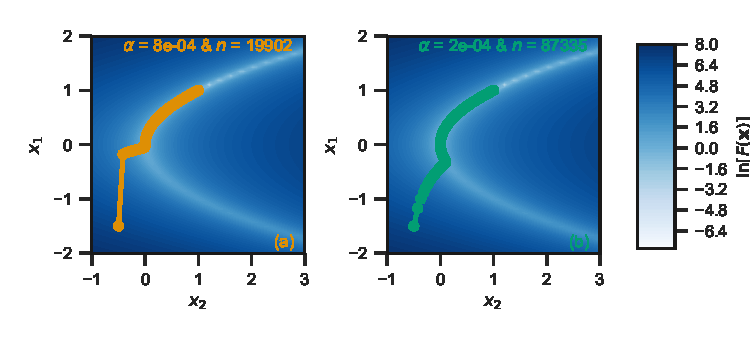
\includegraphics[width=0.85\textwidth]{theory/grad}
    \caption{Example of the gradient descent method applied to a Rosenbrock function \cite{rosenbrock_automatic_1960}, where $a=1$ and $b=100$ (therefore the minima is at ($1$, $1$)), $n$ indicated the number of iterations required to minimise the values. Two different values (\SIlist{2e-4;8e-4}{}) for $\alpha$ are shown to emphasize the efficiency improvement that is possible with the optimisation.}
    \label{fig:grad}
\end{figure}
%
%
\begin{figure}
    \centering
        \lstinputlisting[caption={An example of a simple implementation for the Gradient descent, as applied to a two-dimensional function.},label={cb:grad}]{reports/code_blocks/grad.py}
\end{figure}
%

\subsection{Population optimisation methods}
Population-based algorithms make use of a population of candidate solutions, compared to the single candidate shown in the gradient descent method above.
This population of candidate solutions often have knowledge of the state of each other through some interaction method.
The method of interaction is often used to characterise the algorithms, into evolutionary algorithms (such as differential evolution), and swarm intelligence algorithms (such as the particle swarm method detailed below) \cite{wu_ensemble_2019}.
These population methods are usually more efficient at finding the global minimum for a given search space, than the single candidate methods described above.

\subsubsection{Differential evolution}
\label{sec:de}
Differential evolution (DE) is a common, iterative optimisation algorithm, that was first applied to the analysis of reflectometry and diffraction data by Wormington \emph{et al.} \cite{wormington_characterization_1999}.
Since then, it has proven very popular for the optimisation of reflectometry data and is included in many common analysis programs \cite{bjorck_fitting_2011,bjorck_genx_2007,nelson_co-refinement_2006,nelson_refnx_2019,ott_simulreflec_nodate,kienzle_ncnr_nodate}.
The DE algorithm is designed to more ably determine the global minimum of a particular function \cite{storn_differential_1997}.

DE is an example of a genetic algorithm, one that is designed to mimic the evolution processes observed in biology \cite{holland_adaptation_1992}.
The method consists of two vectors, the parent population, $\mathbf{p}$, the offspring population, $\mathbf{o}$.
These vectors are of a dimension $(i\times j)$, where $i$ is the number of variables being optimised and $j$ is the number of candidate solutions being used.
The offspring population vector is created through some trial methods, many of these exist however we will discuss a simple classical trial method, details of other methods may be found in the work of Bj\"{o}rck \cite{bjorck_fitting_2011}.

A classical trial method consists of two stages, mutation and recombination.
The mutation stage involves performing some mutation on the parent population to create a mutant vector, $\mathbf{m}$, analogous to the mutation in biologically evolutionary theory.
The magnitude of the mutation is dependent on the mutation constant, $k_m$,
%
\begin{equation}
\mathbf{m}_{i,j}= b_{i} + k_m(\mathbf{p}_{i,R1} - \mathbf{p}_{i,R2}),
\end{equation}
%
where $b_{i}$ is the best candidate solution in the parent population, and $\mathbf{p}_{i,R1}$ and $\mathbf{p}_{i,R2}$ are randomly choosen members of the parent population.
The mutation constant can be considered as a control variable for the size of the search radius, with a large $k_m$ corresponding to a larger search radius.

The recombination step creates the offspring population vector by taking a sample from either the parent population or mutant vectors with some frequency, which depends on the recombination constant, $k_r$,
%
\begin{equation}
    \mathbf{o}_{i,j} =
  \begin{cases}
    \mathbf{m}_{i,j}, & \text{where}\ X < k_r \\
    \mathbf{p}_{i,j}, & \text{otherwise}
  \end{cases}
\end{equation}
%
where, $X\sim U[0, 1)$.
The recombination constant controls the progress of the algorithm as it impacts the frequency with which mutation is introduced into the offspring population vector.

The final stage is to compare the offspring and parent population vectors, in the selection stage to create the new parent population for the next iteration.
The selection stage comprises of using some figure of merit, $\zeta$, to choose between the subunit from the offspring or parent population vector.
In our example, that figure of merit may be the agreement between some experimental data and our model, or for the example in Figure~\ref{fig:diff_evo} it is the value of the Ackley function \cite{ackley_connectionist_1987}, which we are trying to minimise.
%
\begin{equation}
    \mathbf{p}_{*,j} \leftarrow
    \begin{cases}
        \mathbf{o}_{*,j}, & \text{where}\ \zeta_{\mathbf{o}_{*,j}} < \zeta_{\mathbf{p}_{*,j}} \\
        \mathbf{p}_{*,j}, & \text{otherwise}
    \end{cases}
\end{equation}
%
where, the $*$ notation indicates all objects in the given population, and $\zeta_{\mathbf{o}_{*,j}}$ and $\zeta_{\mathbf{p}_{*,j}}$ are the figures of merit for the offspring and population population candidate solutions respectively.
%
\begin{figure}
    \centering
    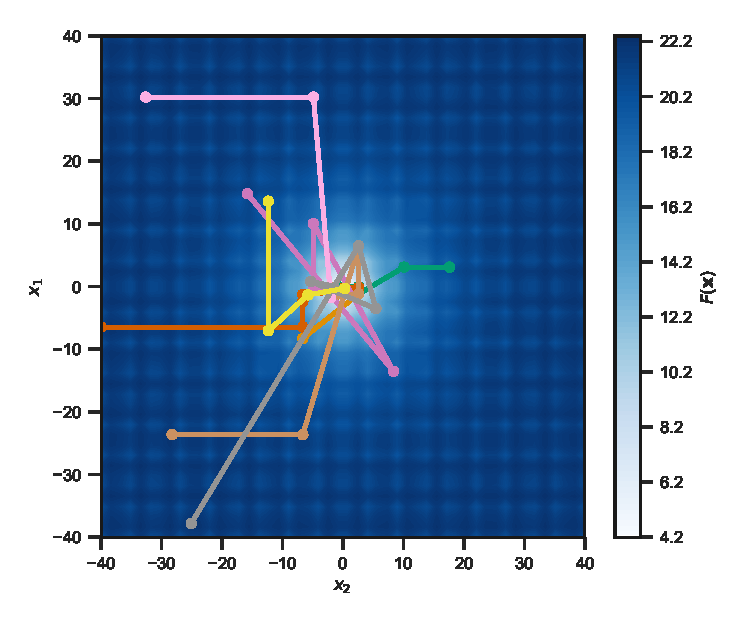
\includegraphics[width=0.85\textwidth]{theory/diff_evo}
    \caption{An example of a differential evolution (DE) algorithm as applied to an Ackley function \cite{ackley_connectionist_1987}, where $a=20$, $b=0.2$, and $c=2\pi$ (a common function for assessing global optimisation methods). The mutation and recombination constant in this implementation are both $0.5$. Each different coloured line represents a different candidate solution. The optimisation was stopped after $100$ iterations had run.}
    \label{fig:diff_evo}
\end{figure}
%

It is noted that it is often the case, in particular, when optimising experimental data, that there should be some bounds applied to the variables within the populations.
However, the DE algorithm may disregard these bounds due to the nature of the mutation step.
Therefore, it is common in DE algorithms, where bounds must be set, that if the search space moves outside that expected it is necessary to reinitialise the parameter.
An implementation of the DE algorithm is given programmatically in Code Block~\ref{cb:diff_evo}, where this reinitialisation is achieved by obtaining a new random number within the given bounds.
%
\begin{figure}
        \lstinputlisting[caption={An example of a simple implementation for a DE algorithm as described by Bj\"{o}rck \cite{bjorck_fitting_2011}.},label={cb:diff_evo}]{reports/code_blocks/diff_evo.py}
\end{figure}
%
%
\begin{figure}
    \centering
        \lstinputlisting[caption={The mutation step used in a classical trial method for a differential evolution algorithm, as described by Bj\"{o}rck \cite{bjorck_fitting_2011}.},label={cb:mut}]{reports/code_blocks/mutation.py}
\end{figure}
%
%
\begin{figure}
    \centering
        \lstinputlisting[caption={The recombination step used in a classical trial method for a differential evolution algorithm, as described by Bj\"{o}rck \cite{bjorck_fitting_2011}.},label={cb:recomb}]{reports/code_blocks/recombination.py}
\end{figure}
%
%
\begin{figure}
    \centering
        \lstinputlisting[caption={The selection step used in a differential evolution algorithm, as described by Bj\"{o}rck \cite{bjorck_fitting_2011}.},label={cb:sel}]{reports/code_blocks/selection.py}
\end{figure}
%

\subsubsection{Particle swarm}
\label{sec:partswarm}
Particle swarm optimisation is a type of swarm intelligence population-based optimisation method.
This optimisation method was originally developed by Kennedy, Eberhart, and Shi for the simulation of social organisms such as bird flocks \cite{kennedy_particle_1995,shi_modified_1998}.
Particle swarm methods are particularly suitable for the optimisation, and sampling, of parametric search-spaces with a large number of similar minima, and therefore is useful for the study of the self-assembly of soft matter materials (Section~\ref{smallangle}).

These methods consist of a population vector, similar to that described for the differential evolution, that moves around the parametric search-space.
The motions of these `particles' are influenced by the positions of the other particles in the vector \cite{poli_analysis_2008}.
It is anticipated that this will lead the swarm to optimise the function under investigation.

Particles in the swarm are under the influence of two elastic forces.
The first attracts the particle to the best location in the search-space that the particle has found, while the other attracts the particle to the best search-space location found by any particle of the swarm.
The magnitudes of these forces are randomised but modulated by a pair of acceleration coefficients, $\psi_p$ that influences the attraction towards the personal best location, and $\psi_g$ that influences the attraction to the global best location.
The position of a particle changes between iterations of the algorithm based on the following relation,
%
\begin{equation}
\mathbf{p}_{*,j} \leftarrow \mathbf{p}_{*,j} + \mathbf{v}_{*,j},
\end{equation}
%
where, $\mathbf{p}_{*,j}$ is the position of the particle, and $\mathbf{v}_{*,j}$ is the velocity of the particle.
This velocity is determined as shown below,
%
\begin{equation}
\mathbf{v}_{*,j} \leftarrow \omega\mathbf{v}_{*,j} + \psi_gR1(\mathbf{g}_{*} - \mathbf{p}_{*,j}) + \psi_pR2(\mathbf{s}_{*,j} - \mathbf{p}_{*,j}),
\end{equation}
%
where, $\omega$ a constant known as the interia weight, $R1\sim U[0, 1)$ and $R2\sim U[0, 1)$ are random numbers, $\mathbf{g}_{*}$ is the best position occupied by any particle in the swarm and $\mathbf{s}_{*,j}$ is the person best for the particle $j$.

Figure~\ref{fig:part_swarm} shows an example of the particle swarm optimisation in action, applied to the Ackley function \cite{ackley_connectionist_1987}. Code Block~\ref{cb:part_swarm} shows a functional programmatic implementation of a particle swarm optimisation algorithm.
%
\begin{figure}
    \centering
    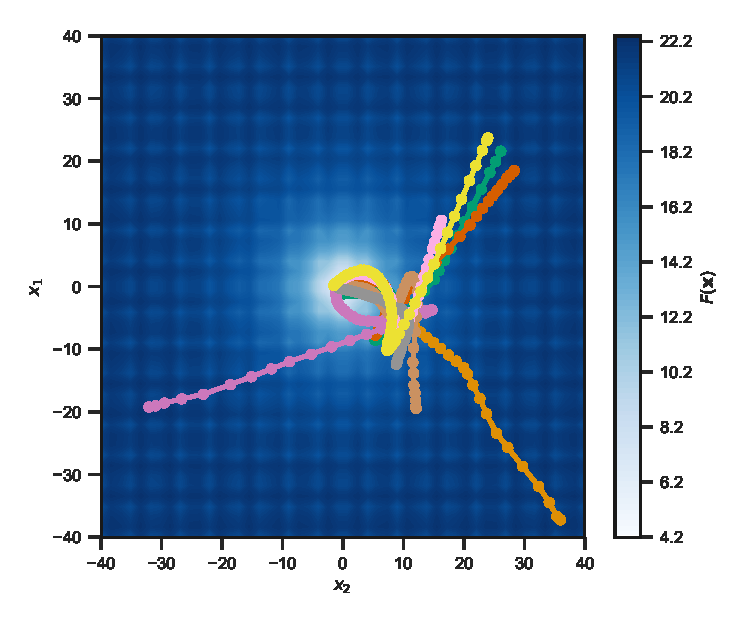
\includegraphics[width=0.85\textwidth]{theory/part_swarm}
    \caption{An example of a particle swarm optimisation as applied to an Ackley function \cite{ackley_connectionist_1987}, where $a=20$, $b=0.2$, and $c=2\pi$. For the particle swarm, the following parameters were used $\omega=0.9$, $\psi_g=0.05$, and $\psi_p=0.05$. Each different coloured line represents a different candidate solution. The optimisation was stopped after $100$ iterations had run.}
    \label{fig:part_swarm}
\end{figure}
%
\begin{figure}
    \centering
        \lstinputlisting[caption={An example of the particle swarm optimisation algorithm \cite{poli_analysis_2008}.},label={cb:part_swarm}]{reports/code_blocks/part_swarm.py}
\end{figure}
%

\subsection{Markov chain Monte-Carlo}
\label{sec:mcmc}
Markov chain Monte-Carlo (MCMC) is a sampling methodology, derived from direct sampling Monte-Carlo \cite{krauth_statistical_2006}.
The aim of an MCMC algorithm is to sample a probability distribution, when parameters are described in terms of their degree of probability \cite{sivia_data_2006}.
Similar to molecular dynamics, in practical terms, MCMC should not be used on a system that is not already optimised, as its purpose is probability distribution sampling rather than minimisation.
Generally, the approach would be to optimise using, for example, one of the approaches described above, then to use MCMC or molecular dynamics to sample the appropriate search-space.
For example, in this work MCMC is used extensively, following the optimisation of a reflectometry model using a differential evolution algorithm, to quantify the inverse uncertainties of the model.
In this context, the inverse uncertainty is the uncertainty on a given parameter within the model.
In addition to being able to give information about the inverse uncertainties, MCMC also offers a more complete understanding of the correlations present between the different parameters \cite{gilks_markov_1995}, as the interactions between the parameter variation has been quantified.

The aim of MCMC is to only sample configurations of a given function that are within the experimental uncertainty.
Figure~\ref{fig:mcmc} shows an example of the possible output that may be obtained from the application of an MCMC sampling method.
This was generated using a Metropolis-Hastings algorithm \cite{metropolis_equation_1953,hastings_monte_1970}, shown in Code Block~\ref{cb:mcmc}.
Initially, a Levenberg–Marquardt algorithm \cite{levenberg_method_1944,marquardt_algorithm_1963} was used to optimise the positions and integral of the two Gaussian functions that make up the data.
The MCMC was used to sample the values that were within the experimental uncertainty.
%
\begin{figure}
    \centering
    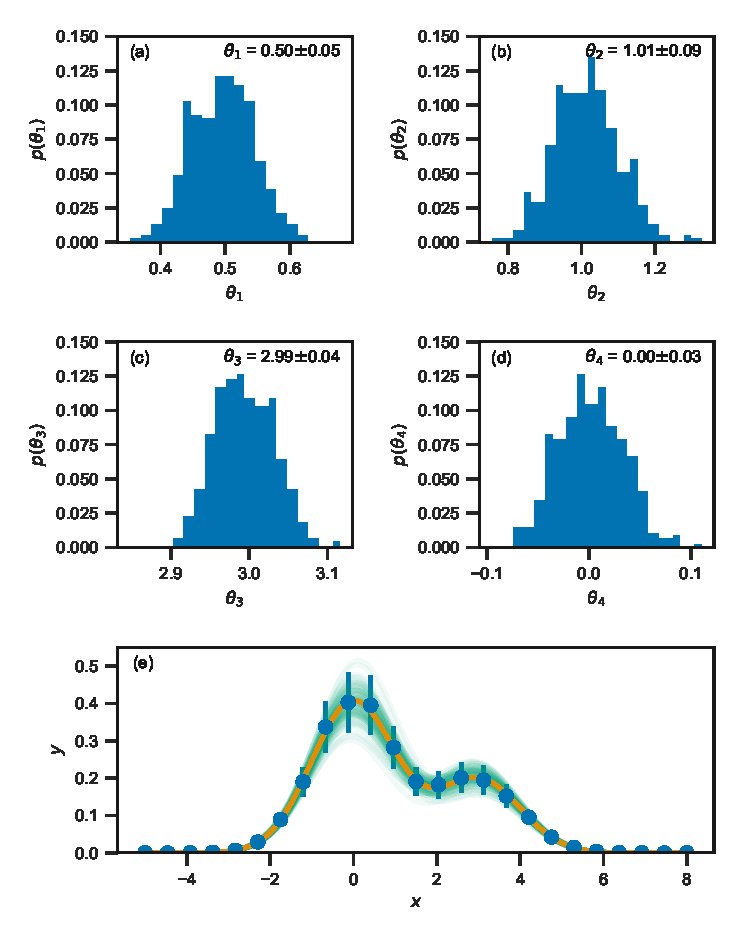
\includegraphics[width=0.85\textwidth]{theory/mcmc}
    \caption{An example of a four variable (two nearby Gaussian functions of different sizes with added random noise and some fractional uncertainty) problem probed using a MCMC method, using values of $a=0.1$, $\theta_1$ and $\theta_2$ correspond to the integral of the Gaussian function, while $\theta_3$ and $\theta_4$ indicate their positions; (a)-(d) histograms of the probability distribution function for each of the varibles, and (e) the data (blue circles), the optimised solution (orange line), and a series of probable solutions (green lines) showing the variability present in the data uncertainty.}
    \label{fig:mcmc}
\end{figure}
%
\begin{figure}
    \centering
        \lstinputlisting[caption={An example of the Metropolis-Hastings MCMC algorithm \cite{metropolis_equation_1953,hastings_monte_1970}.},label={cb:mcmc}]{reports/code_blocks/mcmc.py}
\end{figure}
%

Once an optimised solution, $\theta$, is obtained, the figure of metric is calculated, in Code Block~\ref{cb:mcmc} this is the agreement between the model and the experimental data, $\chi^2$, where,
%
\begin{equation}
\chi^2 = \sum\frac{(y_{\text{exp}} - y_{\text{calc}})^2}{\text{d}y_{\text{exp}}},
\end{equation}
%
and $y_{\text{exp}}$ is the experimental data, and $\text{d}y_{\text{exp}}$ the uncertainty in the experimental data, while $y_{\text{calc}}$ is the model solution.
Some random pertubation is then applied to the optimised solution,
%
\begin{equation}
\Theta = \theta + aR,
\end{equation}
%
where $R\sim N(0, 1)$.
A new $\chi^2$ is found for $\Theta$, and the probablity that this transition will occur is found,
%
\begin{equation}
p = \exp{\bigg(\frac{-\chi^2(\Theta) + \chi^2(\theta)}{2}\bigg)}.
\end{equation}
%
This probability is then compared with a random number $n\sim U[0, 1)$, and if $n$ is less than the probability, the new solution is stored,
%
\begin{equation}
\theta \leftarrow \Theta.
\end{equation}
%
This process is repeated until some desired number of samples has been obtained.
It should be noted that in the event on a poorly optimised initial value of $\theta$, it may be necessary to `burn' (that is to ignore) the first series of solutions while the MCMC algorithm settles into the search-space.

\subsection{Molecular dynamics}
\label{sec:md}
Section \ref{sec:classical} introduced classical potential models as a method for the evalution of the interaction energy of a given chemical system.
Any of the optimisation methods discussed above could be used alongside these classical potential models to find an energy minimum structure for the system or to sample the potential energy landscape.
However, it is often the case that we are interested in a dynamically relevant structure at a given temperature for some system.
This is where molecular dynamics simulations are a useful and important tool.

\subsubsection{Forces and accelertions}
The aim of a molecular dynamics simulation is to probe the positions, velocities, and accelerations on each of the atoms, or coarse-grained particles, as a simulation progresses.
The acceleration on a given particle, $\mathbf{a}$ is defined by the force on that particle, $\mathbf{f}$, in agreement with Newton's second law of motion,
%
\begin{equation}
\mathbf{f} = m\mathbf{a},
\label{equ:forcevec}
\end{equation}
%
where, $m$ is the mass of the particle.
In order to determine the acceleration on the particle, it is necessary to know the force on that particle.
The force, $f$, is a function of the potential energy, $E$, as found from a classical potential, of that atom,
%
\begin{equation}
f(r) = \frac{-\partial E_{\text{total}}(r)}{\partial r},
\label{equ:forcesca}
\end{equation}
%
where, $r$ is the configuration of the atoms.
Which is to say that, the force is the negative of the first derivative of the energy with respect to the atomic configuration.
The force found from Equation~\ref{equ:forcesca} is a scalar, however, we are interested in the force vector in Equation~\ref{equ:forcevec}.
To determine the force in a given direction, it is necessary to find the product of the force, $f$, and the unit vector in that direction,
%
\begin{equation}
\mathbf{f}_x = f\hat{\mathbf{r}}_x, \;\;\;\text{where}\;\hat{\mathbf{r}}_x = \frac{r_x}{|\mathbf{r}|},
\end{equation}
%
where $r_x$ is the atomic configuration in the $x$-dimension, and $|\mathbf{r}|$ is the magnitude of the atomic configuration vector.

\subsubsection{Integration}
The potential model, which we define for a given system, allows for the calculation of the acceleration on each particle in that system.
The next step is to use this acceleration to iterate through the trajectory of our system.
This is achieved by applying Newtonian equations of motion, for example in the Velocity-Verlet algorithm \cite{swope_computer_1982}.
%
\begin{equation}
\mathbf{x}(t + \Delta t) = \mathbf{x}(t) + \mathbf{v}(t)\Delta t + \frac{1}{2}\mathbf{a}(t)\Delta t^2, \\
\label{equ:vv1}
\end{equation}
\begin{equation}
\mathbf{v}(t + \Delta t) = \mathbf{v}(t) + \frac{1}{2}\big[\mathbf{a}(t) + \mathbf{a}(t+\Delta t)\big]\Delta t,
\label{equ:vv2}
\end{equation}
%
where, $\mathbf{x}$ is the position the particle $\mathbf{v}$ is the particle's velocity, and $\mathbf{a}$ is the particle's acceleration, while $t$ is current simulation time and $\Delta t$ is the timestep.
These equations constitute the Velocity-Verlet algorithm,
%
\begin{enumerate}
\item calculate the force (and therefore the acceleration) on each particle (Equations~\ref{equ:forcevec} \& \ref{equ:forcesca}),
\item find the position of the particle after some timestep (Equation~\ref{equ:vv1}),
\item determine the new velocity for each particle, based on the average acceleration at the current and new positions (Equation~\ref{equ:vv2}),
\item overwrite the old acceleration values with the new ones,
\item go to 1.
\end{enumerate}
%
Following an equilibration period, this algorithm may be iterated as many times as is required to obtain sufficient statistics for the measurement quantity of interest, e.g. particle positions for structural techniques such as elastic scattering.

The above analytical process is known as the integration step, and the Velocity-Verlet is the integrator.
If the size of the timestep $\Delta t$ is too large, the step size for a given iteration will not be accurate, as the forces on the atoms will change too significantly during it.
Therefore, the values of the timestep is usually on the order of \SI{10e-15}{\second} (\si{\femto\second}).
This means that in order to simulate a single nanosecond of ``real-time'' molecular dynamics, the integrator must be solved one million times.
This can be slow for very large systems, leading to an interest in coarse-grained simulations that result in fewer particles to determine the forces for (speeding up the integration step), but also enable to use of larger timesteps (so fewer integrations must be solved) \cite{rudd_coarse-grained_1998,brini_systematic_2013}, for example, the use of a MARTINI potential model allows for an upto twenty times increase in the timestep compared to an all-atom model.

\subsubsection{Initialisation}
The above discussion ignored two aspects that are necessary to run a molecular dynamics simulation, both of which as associated with the original configuration of the system; the original particle positions and velocities.

The particle positions are usually taken from some library, for example for the simulation of a protein, often the protein data bank \cite{noauthor_rcsb_nodate} is a useful resource.
Small molecules may be configured by hand using graphical programs such as Jmol \cite{noauthor_jmol_nodate}.
These small molecules may be built into complex, multicomponent structures using software such as the Packmol package \cite{martinez_packmol_2009}.
The importance of this initial structure cannot be overstated, for example, if the initial structure in a molecular dynamics simulation is unrepresentative of the equilibrium structure, it may take a large amount of simulation time before the equilibrium structure is obtained, possibly much longer than could be reasonably simulated.

The initial particle velocities are obtained in a much more general fashion.
They are selected randomly, and then scaled such that the kinetic energy, $E_K$, of the system agrees with a defined temperature, $T$,
%
\begin{equation}
E_K = \sum_{i=1}^N{\frac{m_i|\mathbf{v}_i|^2}{2}} = \frac{3}{2}Nk_BT,
\label{equ:ek}
\end{equation}
%
where, $m_i$ and $\mathbf{v}_i$ are the masses and velocities of the particles, $N$ is the number of particles, and $k_B$ is the Boltzmann constant.

\subsubsection{Ensembles}
The above algorithm details a simulation that makes use of an NVE ensemble, a simulation where the number of particles (N), the volume of the system (V), the energy of the system (E) are all kept constant.
However, this is not the only simulation ensemble that is available, within this work two other ensembles have been used extensively,
%
\begin{itemize}
\item the NVT (canonical) ensemble; this is similar to the NVE ensemble except the simulation temperature is controlled via a thermostat,
\item the NPT (isothermal-isobaric); this ensemble is similar to the NVT ensemble, however, the system volume is allowed to vary while the overall system pressure is held constant using a barostat.
\end{itemize}
%
Thermostating involves controlling the kinetic energy of the particles (Equation~\ref{equ:ek}) such that the simulation temperature is kept at a predefined value.
There are a variety of methods for thermostating a molecular dynamics simulation, such as the Andersen, Nos\'{e}-Hoover, or Berendsen methods \cite{andersen_molecular_1980,nose_unified_1984,berendsen_molecular_1984,hoover_canonical_1985}.
However, the most straightforward to describe, and that implemented in the \texttt{pylj} software (discussed in detail in Chapter \ref{teaching}) \cite{mccluskey_pylj_2018,mccluskey_arm61/pylj_2018} is a velocity rescaling \cite{bussi_canonical_2007}.
This is where the velocities for a random subset of the particles, $\mathbf{v}_i$ are adapted based on the following relation,
%
\begin{equation}
\mathbf{v}_i \leftarrow \mathbf{v}_i \sqrt{\frac{T_{\text{target}}}{\bar{T}}}
\end{equation}
%
where, $T_{\text{target}}$ is the target temperature, and $\bar{T}$ is the average simulation temperature.

The use of a barostat to control the simulation pressure usually involves varying the simulation cell parameters and the distances between the particles.
This would in a similar way to thermostating, where the simulation dimensions are scaled by a value in an effort to control the pressure.
The barostating methods are similar to the thermostating methods with Andersen, Nos\'{e}-Hoover, and Berendsen methods.
However, there is also the Parrinello-Rahman barostat which allows for independent control of the different cell dimensions giving control of stress in addition to pressure \cite{parrinello_polymorphic_1981}.

These optimisation and sampling methods were used in a variety of different applications within this work, firstly differential evoluation optimisation and MCMC sampling are used in Chapter~\ref{reflectometry1} in the study of a chemically-consistent modelling approach to X-ray and neutron reflectometry analysis.
Molecular dynamics simulation are investigated as a possible tool to assist in the analysis of reflectometry in in Chapter~\ref{reflectometry2}.
Finally, the particle swarm optimisation is applied for the efficient determination of a micelle structure for ftting small angle scattering data in Chapter~\ref{smallangle}.
